\chapter{Exchanges, Order Types, and the Limit Order Book}
\label{ch:lob}
\chaptermark{Exchanges and the LOB}

A market is a crowd of buyers and sellers, each with a different view
of what something is worth, trying to find each other without knowing
who is on the other side, without wanting to wait, and without
trusting each other to hold an order until it matches.
\emph{How do you engineer a fair, fast, rule-based mechanism that
pairs them off without missing any willing trade?} The answer
dominates this chapter and every chapter that follows: the
\textbf{limit order book} (LOB), a simple data structure that every
professional trading venue converges on, and the \textbf{matching
engine} that operates on it. This chapter defines the vocabulary
(bid, ask, spread, order types, maker/taker, tick size) that every
later chapter assumes. Nothing here is mathematically deep, but every
bold term is load-bearing.

\begin{backgroundbox}[Prerequisites]
This is the first content chapter; no prior chapters are required.
From outside the book the reader should bring:
\begin{itemize}
  \item \textbf{Programming.} Ability to read a Python snippet using a
  sorted data structure and plain-old objects. No library-specific
  knowledge required.
  \item \textbf{Real world.} Passing awareness that stocks trade on
  exchanges. Zero finance background is assumed; every technical term
  below is defined on first use.
\end{itemize}
\end{backgroundbox}

\section{Double-sided auctions}
\label{sec:double_sided}

An \textbf{exchange} is a venue (nowadays almost always software in
a colocation data centre) whose only job is to accept messages
called \emph{orders}, match buyers with sellers according to a fixed
published rule, and report the resulting trades. A \textbf{product} is
whatever is being traded; think of a stock, but it could equally be a
bond, a futures contract, a Prosperity \texttt{RAINFOREST\_RESIN}, or
a kilo of coffee. The exchange runs one such auction per product, in
parallel, continuously. Because a product has both buyers and sellers
at any instant, the mechanism is a \emph{double-sided auction}, as
opposed to a one-sided auction like eBay, where bids are collected
against a single seller.

\begin{historybox}
Before the late 1990s a ``double-sided auction'' meant a physical
\emph{pit}: human traders shouting bids and asks in hand signals.
The NYSE ran its floor this way from 1792; the CBOT and LIFFE kept
their pits through the 1990s. Electronic matching arrived gradually:
NASDAQ's SelectNet (1988), the Swiss Exchange fully electronic
(1996), the LSE abandoning its floor (1997), Eurex absorbing the
Deutsche Terminb\"orse (1998). By about 2010 equity and
futures volume was essentially all electronic. The mental model of
this chapter, orders as messages and the book as a data structure,
only became universally applicable in the last two decades; before
that, a crowd of humans approximated the same data structure by
shouting. Harris \citeHarris{} gives the long version.
\end{historybox}

The two sides of the auction get names:

\begin{itemize}
  \item A \textbf{bid} is a willingness to buy at a specified price.
  Synonyms: ``buy order'', ``bid order''. The highest bid price
  currently resting in the market is the \textbf{best bid}, written
  $\bidp$.
  \item An \textbf{ask} (also \textbf{offer}) is a willingness to sell
  at a specified price. Synonyms: ``sell order'', ``ask order''. The
  lowest ask price currently resting in the market is the
  \textbf{best ask}, written $\askp$.
\end{itemize}

The gap between them is the \textbf{spread}, $\spreads = \askp -
\bidp$. The arithmetic average of the two is the \textbf{mid}
(sometimes \emph{mid-price}), $\midp = (\bidp + \askp)/2$. A trade
happens when someone sends a new order that \emph{crosses} the book:
a buy at or above $\askp$, or a sell at or below $\bidp$. Until then,
no trade; the orders simply sit and wait.

Why is $\bidp < \askp$ at all? If someone will sell at $103.23$ and
someone else will buy at $102.54$, isn't a trade missing? No: it
means \emph{no one} was willing to buy at $103.23$ or higher, and
\emph{no one} was willing to sell at $102.54$ or lower. The spread is
the signature of that fact. \Cref{ch:spreads_roll} shows that a
strictly positive spread is forced on any real market by inventory
risk, order-processing cost, and adverse selection; for now, take a
non-zero spread as an empirical fact.

\begin{keyfactbox}[Bid/ask/spread/mid]
\begin{align*}
  \bidp &\;=\; \text{highest buy price resting in the book}, \\
  \askp &\;=\; \text{lowest sell price resting in the book}.
\end{align*}
\[
  \spreads \;\defeq\; \askp - \bidp \;\geq\; 0, \qquad
  \midp \;\defeq\; \tfrac{1}{2}(\bidp + \askp).
\]
These four numbers are the minimum summary of a market's current
state. \emph{None} of them is ``the price'' of the product; that
ambiguity is the subject of \cref{ch:price_value}, which introduces
five more candidates.
\end{keyfactbox}

Here is a toy limit order book with four price levels per side. The
\emph{bid side} is sorted with highest price at top (best for a
seller); the \emph{ask side} with lowest price at top (best for a
buyer).

\begin{figure}[ht]
\centering
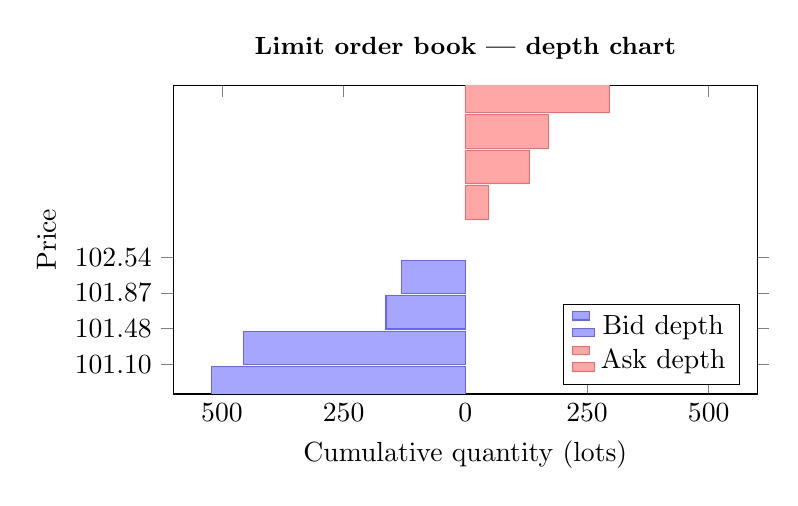
\begin{tikzpicture}
\begin{axis}[
  xbar, bar width=12pt,
  width=9cm, height=5.5cm,
  xlabel={Cumulative quantity (lots)},
  ylabel={Price},
  symbolic y coords={101.10,101.48,101.87,102.54,103.23,103.98,104.17,104.75},
  ytick=data,
  xmin=-600, xmax=600,
  xtick={-500,-250,0,250,500},
  xticklabels={500,250,0,250,500},
  title={Limit order book --- depth chart},
  title style={font=\small\bfseries},
  legend pos=south east,
  enlarge y limits=0.12,
]
\addplot[fill=blue!35, draw=blue!60]
  coordinates {(-131,102.54) (-163,101.87) (-456,101.48) (-521,101.10)};
\addplot[fill=red!35, draw=red!60]
  coordinates {(48,103.23) (132,103.98) (170,104.17) (297,104.75)};
\legend{Bid depth, Ask depth}
\end{axis}
\end{tikzpicture}
\caption{Limit order book depth chart for the toy book tabulated
below. Bid-side bars (blue) extend leftward; ask-side bars (red)
extend rightward. The best bid is $102.54$ and the best ask is
$103.23$, giving a spread of $0.69$. Each bar shows the cumulative
resting quantity at that price level and all levels behind it.}
\label{fig:lob_depth_chart}
\end{figure}

\begin{center}
\begin{tabular}{cc|cc}
\toprule
\multicolumn{2}{c|}{\textbf{BID SIDE}} & \multicolumn{2}{c}{\textbf{ASK SIDE}} \\
Qty & Price & Price & Qty \\
\midrule
$131$ & $102.54$ & $103.23$ & $48$ \\
$32$  & $101.87$ & $103.98$ & $84$ \\
$293$ & $101.48$ & $104.17$ & $38$ \\
$65$  & $101.10$ & $104.75$ & $127$ \\
\bottomrule
\end{tabular}
\end{center}

For this book, $\bidp = 102.54$, $\askp = 103.23$, $\spreads = 0.69$,
$\midp = 102.885$. A new limit buy at $102.00$ does \emph{not} cross
(below the best ask) and rests on the bid side between $102.54$ and
$101.87$. A new market buy executes immediately against the $48$
shares at $103.23$, then continues into $103.98$ if its size exceeds
$48$. That ``eating into the book'' behaviour is the central risk of
\cref{sec:order_types}, worked through below.

\section{Order types}
\label{sec:order_types}

An \textbf{order} is a message to the exchange: ``I want to trade,
and here is how.'' Every order carries a \emph{side} (buy or sell), a
\emph{quantity}, and a \emph{product}. Beyond that, orders differ by
\emph{when} they execute, at \emph{what} price, and for \emph{how
long} they remain active. The set below is the core vocabulary; every
real exchange supports all of them, and Prosperity supports the first
two.

\begin{definition}[Limit order]
\index{limit order|textbf}\index{order!limit|textbf}
A \emph{limit order} is an order to buy up to $q$ units at a price no
higher than $p$, or to sell up to $q$ units at a price no lower than
$p$. If it can be matched immediately against the resting book, it
is; whatever quantity cannot be matched rests as a new entry in the
book. A limit order with $p$ set such that it crosses the best quote
on the other side is called \emph{marketable}.
\end{definition}

Limit orders are the fundamental object; every other order type is a
limit order with an extra constraint on price or time-in-force.

\begin{definition}[Market order]
\index{market order|textbf}\index{order!market|textbf}
A \emph{market order} is an order to buy or sell $q$ units
\emph{immediately} at whatever prices are available, sweeping from the
best quote outward until $q$ units are filled. Equivalently (the
cleanest implementation in the Python section below), a market buy
is a limit buy with $p = +\infty$, and a market sell is a limit sell
with $p = 0$.
\end{definition}

\begin{definition}[Immediate-or-cancel (IOC)]
\index{immediate-or-cancel (IOC)|textbf}\index{IOC|textbf}\index{order!IOC|textbf}
An \emph{IOC} order behaves like a limit order, but any portion that
cannot be matched immediately is cancelled rather than resting in the
book. Used by takers who do not want to leave a resting quote behind.
Typical use: a strategy sweeps the best ask with a capped price to
take available size now, without risk of the unfilled remainder
sitting in the book and being picked off if the mid moves against it a
moment later.
\end{definition}

\begin{definition}[Fill-or-kill (FOK)]
\index{fill-or-kill (FOK)|textbf}\index{FOK|textbf}\index{order!FOK|textbf}
An \emph{FOK} order executes in full immediately, or not at all. If
the full quantity $q$ cannot be filled against the current book, the
exchange rejects the order entirely and no partial fill is reported.
Used when partial fills are operationally costly, for example
a hedge that is only valid as one unit.
\end{definition}

Three further order types complete the core vocabulary. They are less
fundamental (you won't need them algorithmically in this book) but
every practitioner is expected to know them. A \textbf{stop order} is
dormant until the last traded price crosses a \emph{trigger} $p_s$,
at which point it becomes a market order (or a limit order, for a
\emph{stop-limit}); the classic example is a stop-loss sell: ``if
the price drops to $p_s$, sell me out.'' A \textbf{hidden order} is a
resting limit order the exchange will match against but does not
publish in public book data; the trader loses price--time priority
against visible orders at the same level in exchange for invisibility.
An \textbf{iceberg order} is a large limit order whose total size is
hidden but which publishes a small \emph{tip}; each time the tip is
consumed, the exchange reveals another slice of the same size. Used
by institutions that need to transact size without announcing it.

Orthogonal to the order type, every real exchange attaches a
\textbf{time-in-force (TIF)} flag saying \emph{how long} a resting
order should live if it does not match immediately. The three you
will see everywhere:

\begin{itemize}
  \item \textbf{DAY.} Cancels at session end. The default on most
  equity venues.
  \item \textbf{GTC (Good-till-cancelled).} Rests across sessions
  until the participant cancels or the order trades. Used by passive
  strategies that persist through overnight breaks.
  \item \textbf{GTD (Good-till-date).} Cancels at a specified future
  timestamp. Useful when an order is conditional on an event whose
  relevance expires.
\end{itemize}

IOC and FOK are technically TIFs too: ``cancel the unfilled remainder
now'' and ``cancel the whole order now if it cannot fill in full''.
Prosperity orders behave as ``immediate only'': they match in the
current tick or are cancelled when the next \texttt{TradingState}
arrives (\cref{sec:first_prosperity}).

The key distinction to internalise (limit vs market vs IOC/FOK)
controls whether an order \emph{provides} liquidity (rests) or
\emph{consumes} it (hits something resting). \Cref{sec:makers_takers}
turns that split into the maker/taker dichotomy that runs through the
whole book.

\begin{pitfallbox}[Market orders can slip through a thin book]
A market buy sent into a visible best ask of $103.23$ does \emph{not}
guarantee an execution price of $103.23$. Take the toy book from
\cref{sec:double_sided} verbatim:
\begin{center}
\begin{tabular}{cc|cc}
\toprule
\multicolumn{2}{c|}{BID SIDE} & \multicolumn{2}{c}{ASK SIDE} \\
Qty & Price & Price & Qty \\
\midrule
$131$ & $102.54$ & $103.23$ & $48$  \\
$32$  & $101.87$ & $103.98$ & $84$  \\
$293$ & $101.48$ & $104.17$ & $38$  \\
$65$  & $101.10$ & $104.75$ & $127$ \\
\bottomrule
\end{tabular}
\end{center}
Send a market buy for $200$ shares. The ask side has only $48 + 84 +
38 = 170$ shares at or below $104.17$, so the first three levels fill
in full and the fourth absorbs the remaining $30$ shares at $104.75$:
\[
\underbrace{48 \times 103.23}_{\text{level 1}} +
\underbrace{84 \times 103.98}_{\text{level 2}} +
\underbrace{38 \times 104.17}_{\text{level 3}} +
\underbrace{30 \times 104.75}_{\text{level 4}}
= 20{,}790.32.
\]
Average execution price is $20{,}790.32 / 200 = 103.9516$, about $72$
cents ($\sim 70$ basis points) above the best ask of $103.23$. The
gap between top-of-book quote and realised average fill is
\textbf{slippage}. In a thin book, slippage from one aggressive market
order can dwarf a strategy's edge. The standard defence is a
marketable limit with a price cap (e.g.\ $103.50$), accepting a
partial fill rather than a bad full one. \Cref{ch:market_impact}
treats slippage as a systematic cost and shows it scales empirically
as $\sqrt{Q}$ on liquid venues.
\end{pitfallbox}

\section{The limit order book as a data structure}
\label{sec:lob_ds}

Stripped of exchange-specific packaging, a limit order book is two
sorted lists of resting limit orders, one per side.

\begin{definition}[Limit order book]
\index{limit order book (LOB)|textbf}\index{order book|textbf}\index{LOB|textbf}
A \emph{limit order book} (LOB) for a product is the pair of
multisets
\[
  B_t \;=\; \{(\mathrm{price}_i, \mathrm{qty}_i, \mathrm{time}_i)\},
  \qquad
  A_t \;=\; \{(\mathrm{price}_j, \mathrm{qty}_j, \mathrm{time}_j)\},
\]
of resting buy (\emph{bid}) and sell (\emph{ask}) limit orders at time
$t$, respectively. $B_t$ is conventionally sorted by price descending
then time ascending; $A_t$ is sorted by price ascending then time
ascending. We require $B_t$ and $A_t$ to be \emph{uncrossed}: every
bid price is strictly below every ask price.
\end{definition}

\begin{definition}[Price--time priority]
\index{price-time priority|textbf}
An exchange uses \emph{price--time priority} if an incoming marketable
order is filled first against the resting order with the most
attractive price for the incoming side, and if several orders share
that price, against the one that arrived first. In other words, the
matching engine consumes orders in exactly the order they appear in
the sorted LOB above.
\end{definition}

Price--time priority is the dominant rule. The main alternative is
\textbf{pro-rata matching}, where at a given price level an incoming
order is split proportionally by size across resting orders: resting
orders of $300$ and $100$ at $102.54$ would receive $75\%$ and $25\%$
of any incoming fill. Pro-rata is used on some futures markets
(notably CME short-term interest rate futures) because it encourages
participants to post \emph{large} resting orders; under price--time
priority only the first resting order in queue gets filled, which
rewards speed not size.

\begin{keyfactbox}[Two matching rules]
\textbf{Price--time priority.} Best price wins; ties broken by
arrival time. Rewards speed. Used by NASDAQ, NYSE, LSE, every equity
ECN, and by Prosperity's exchange throughout all four years of the
competition.

\vspace{0.4em}
\textbf{Pro-rata.} Best price wins; ties split proportionally by
resting size. Rewards posted size, not speed. Used on certain
large-lot futures venues (CME Eurodollars, short sterling).

\vspace{0.4em}
\textbf{This book assumes price--time priority throughout} unless a
chapter explicitly says otherwise. Every result in \cref{ch:market_making}
and \cref{ch:order_flow} about queue position assumes price--time
priority.
\end{keyfactbox}

\begin{intuitionbox}
A limit order book is two sorted lists. That's it. Everything people
call ``the market'' (depth, spread, mid, slippage, impact, adverse
selection, market making, queue position, BBO feeds, the entire
vocabulary of HFT) is built from manipulations of those two lists.
Parts~II and~III of this book are, at bottom, an attempt to explain
what those two lists look like, why they look that way, and how to
trade against them.
\end{intuitionbox}

\section{The matching engine: a worked example}
\label{sec:matching_worked}

We play out a sequence of events on a concrete book so the previous
section's rules stop being abstract. This is the chapter's central
worked example, reproduced with minor edits from Pelgrims's
matching-engine blog post \citep{pelgrims2020matching}. Read it with
a pen.

\subsection{Step 1: initial book}

The book starts in the same state as the toy example from
\cref{sec:double_sided}:

\begin{verbatim}
               LIMIT ORDER BOOK
          BID SIDE            ASK SIDE
     QUANTITY    PRICE   PRICE    QUANTITY
    [131.00  -  102.54 | 103.23  -   48.00]
    [ 32.00  -  101.87 | 103.98  -   84.00]
    [293.00  -  101.48 | 104.17  -   38.00]
    [ 65.00  -  101.10 | 104.75  -  127.00]
\end{verbatim}

$\bidp = 102.54$, $\askp = 103.23$, $\spreads = 0.69$. Nothing is
crossing; the matching engine has no work to do.

\subsection{Step 2: two limit buys post}

A first participant submits a limit buy for $24$ shares at $102.55$.
That is better than the current best bid of $102.54$ and does not
cross the ask ($102.55 < 103.23$). The engine finds no cross and
inserts the order at the top of the bid side.

A second participant submits a limit buy for $14$ shares at
$102.55$, the same price, so it does not improve or cross. Under price--time
priority it queues \emph{behind} the $24$-share order. The book is
now:

\begin{verbatim}
          BID SIDE            ASK SIDE
     QUANTITY    PRICE   PRICE    QUANTITY
    [ 24.00  -  102.55 | 103.23  -   48.00]
    [ 14.00  -  102.55 | 103.98  -   84.00]
    [131.00  -  102.54 | 104.17  -   38.00]
    [ 32.00  -  101.87 | 104.75  -  127.00]
\end{verbatim}

The two $102.55$ entries are drawn on separate lines for clarity, but
at the exchange they sit in a single FIFO queue at that price: the
$24$-share order first, the $14$-share order second.

\subsection{Step 3: a limit sell arrives and crosses}

A third participant sends a limit sell for $40$ shares at $102.55$.
This price is \emph{at} the best bid of $102.55$, so the order is
marketable. The matching engine runs its fill loop:

\begin{enumerate}
  \item \textbf{Level 1.} Top of the bid side: $24$ at $102.55$. The
  incoming sell wants $40$; this order supplies $24$. Print trade
  $24 \times 102.55$, remove. Remaining incoming: $16$.
  \item \textbf{Level 1 (continued).} Next in FIFO at $102.55$: $14$
  shares. Print trade $14 \times 102.55$, remove. Remaining: $2$.
  \item \textbf{Level 2?} Next bid is $131$ at $102.54$. The sell's
  limit is $102.55 > 102.54$, so it will not cross further. Stop.
  \item \textbf{Post remainder.} The $2$ unfilled shares rest on the
  ask side at $102.55$, a new best ask (below the previous $103.23$).
\end{enumerate}

Total traded in this event: $38$ shares at $102.55$ across two
trades. The book state after the dust settles:

\begin{verbatim}
          BID SIDE            ASK SIDE
     QUANTITY    PRICE   PRICE    QUANTITY
    [131.00  -  102.54 | 102.55  -    2.00]
    [ 32.00  -  101.87 | 103.23  -   48.00]
    [293.00  -  101.48 | 103.98  -   84.00]
    [ 65.00  -  101.10 | 104.17  -   38.00]
\end{verbatim}

Best bid slips back to $102.54$, best ask jumps down to $102.55$,
spread collapses from $0.69$ to $0.01$. A snapshot feed with
one-second resolution would show only that the mid dropped by about
thirty-five cents, missing the four events that produced it.

\begin{intuitionbox}
Every order-book event, however exotic, is some combination of three
operations you just saw: \emph{insert a new resting order}, \emph{match
against resting orders until quantity or price runs out}, and
\emph{remove consumed orders}. The matching engine does these three
things deterministically, in a fixed priority order, millions of times
per second, for every product listed.
\end{intuitionbox}

\section{A Python matching engine}
\label{sec:matching_engine_py}

The code below is a stripped-down version of the reference matching
engine from Pelgrims's blog. It keeps only what's needed to reproduce
the worked example: an \texttt{Order}, a \texttt{Trade}, an
\texttt{OrderBook} with two sorted lists, and a \texttt{match} method
implementing the Step~3 fill loop. Not production code (no threading,
error handling, cross-trader accounting, or feed publication), just
enough to \emph{run} the example.

\begin{lstlisting}[language=Python, caption={Minimal price--time-priority matching engine. Adapted from \citep{pelgrims2020matching}.}]
from dataclasses import dataclass
from sortedcontainers import SortedList

@dataclass
class Order:                  # +inf price => market buy; 0 => market sell
    side: str; price: float; qty: int

@dataclass
class Trade:
    price: float; qty: int

class OrderBook:
    def __init__(self):
        # Real engines add a sequence counter to break price ties by
        # arrival order; omitted here for brevity.
        self.bids = SortedList(key=lambda o: (-o.price,))   # high to low
        self.asks = SortedList(key=lambda o: ( o.price,))   # low  to high

    def match(self, incoming: Order) -> list[Trade]:
        book = self.asks if incoming.side == 'buy' else self.bids
        crosses = (lambda r: r.price <= incoming.price) if incoming.side == 'buy' \
                  else (lambda r: r.price >= incoming.price)
        trades, consumed = [], []
        for resting in book:
            if incoming.qty == 0 or not crosses(resting): break
            fill = min(incoming.qty, resting.qty)
            trades.append(Trade(resting.price, fill))
            incoming.qty -= fill; resting.qty -= fill
            if resting.qty == 0: consumed.append(resting)
        for r in consumed: book.remove(r)
        if incoming.qty > 0:                                 # rest remainder
            (self.bids if incoming.side == 'buy' else self.asks).add(incoming)
        return trades
\end{lstlisting}

\begin{intuitionbox}
The \texttt{price} field comment (``+inf for a market buy, 0 for a
market sell'') is the whole point of the listing. A market buy is
a limit buy with $p = +\infty$: the crossing predicate
``$r.\mathrm{price} \leq \mathrm{incoming}.\mathrm{price}$'' is true
for \emph{every} resting sell, so the fill loop eats levels until
quantity or book is exhausted. Market sells collapse to limit sells
with $p = 0$ the same way. The seven-line \texttt{match} method
therefore handles all four of $\{\text{limit, market}\} \times
\{\text{buy, sell}\}$ with no special cases. A generic mechanism that
degenerates into familiar special cases at the parameter limits is a
pattern you will see again, especially in \cref{ch:black_scholes}.
\end{intuitionbox}

\section{The order lifecycle}
\label{sec:lifecycle}

From the instant a participant hits ``send'' to the instant cash and
shares change hands, an order passes through a fixed sequence of
states. Different exchanges publish different subsets of these states
and use slightly different names, but the skeleton is universal.

\begin{enumerate}
  \item \textbf{Submit.} The trading system builds the order message
  (side, price, quantity, product, flags) and sends it to the
  exchange gateway.
  \item \textbf{Accept.} The gateway performs cheap sanity checks
  (valid product? valid side? price within the day's collar? margin
  or position limit OK?) and either admits the order to the matching
  engine or rejects it.
  \item \textbf{Rest or match.} The engine checks for a cross. If
  none, the order is inserted at its price--time position and
  \emph{rests}. Otherwise, the \cref{sec:matching_engine_py} fill
  loop runs and produces trades.
  \item \textbf{Partial or full fill.} A fully-filled order leaves
  the book. On a partial fill, the remainder rests (plain limit),
  cancels (IOC), or the whole order is retroactively cancelled
  (FOK).
  \item \textbf{Clear.} The clearing system reports to a clearing
  house: ``$A$ bought $q$ at $p$ from $B$.'' The clearing house
  typically becomes the central counterparty, so $A$ and $B$ never
  need to trust each other directly.
  \item \textbf{Settle.} One or two business days later ($T{+}2$ for
  most equities, $T{+}1$ for US Treasuries, $T{+}0$ for intraday
  futures), the clearing house moves cash and shares irrevocably.
  Only now does the trade economically \emph{exist}.
\end{enumerate}

For strategy content you will rarely care about steps~5 and~6: on
Prosperity both happen instantly, and on a sell-side desk the Strat
role touches post-trade infrastructure little. But know the names:
every real trading system logs events at every stage, and you will
read those logs when debugging.

\begin{keyfactbox}[Order lifecycle]
\textbf{Submit} $\to$ participant sends the order message.
\textbf{Accept} $\to$ gateway validates and admits it.
\textbf{Rest or match} $\to$ engine either posts it or runs the fill
loop. \textbf{Partial or full fill} $\to$ some or all of the quantity
is traded; remainder handled per time-in-force flag.
\textbf{Clear} $\to$ clearing house records the obligation.
\textbf{Settle} $\to$ cash and shares actually move.
\end{keyfactbox}

\section{Makers and takers}
\label{sec:makers_takers}

Every trade has two sides: the \textbf{maker} of liquidity (whose
order was already resting) and the \textbf{taker} of liquidity (whose
incoming order crossed the book). These roles play different economic
games, and exchanges price them differently to influence behaviour.

\begin{definition}[Maker and taker]
\index{maker|textbf}\index{taker|textbf}\index{maker and taker|textbf}
In a trade, the \emph{maker} is the participant whose limit order
was already resting in the LOB when the match occurred; the
\emph{taker} is the participant whose marketable order (limit,
market, IOC, or FOK) crossed the book and triggered the match. By
construction, makers provide liquidity by posting quotes; takers
consume liquidity by hitting them.
\end{definition}

Exchanges want a deep, tight book: it attracts more traders, more
volume, and more fees. But someone has to \emph{post} the resting
orders, and that someone is exposed to adverse selection, inventory
risk, and opportunity cost. The standard solution is a
\textbf{maker--taker fee schedule}: the exchange \emph{charges} the
taker and \emph{pays} the maker (a ``rebate''). Both are small
fractions of notional; the difference is the exchange's cut.

Concrete example. An exchange charges takers $0.30$ basis points
(bps) of notional and pays makers a rebate of $0.20$~bps (where
$1\text{ bp} = 10^{-4} = 0.01\%$). Alice rests a buy limit of $1{,}000$
shares at \$50.00. Bob sends a marketable sell and fills it. Trade
notional: $1{,}000 \times 50 = \$50{,}000$. Then:

\begin{itemize}
  \item Bob (taker) pays a fee of $\$50{,}000 \times 0.30 \text{ bps}
  = \$1.50$ plus the $\$50{,}000$ he owes Alice.
  \item Alice (maker) receives a rebate of $\$50{,}000 \times 0.20
  \text{ bps} = \$1.00$ plus the $\$50{,}000$ Bob owes.
  \item The exchange pockets the difference, $\$0.50$.
\end{itemize}

The rebate of \$1.00 on \$50{,}000 is tiny: two ten-thousandths
of a percent. For a strategy that crosses the spread once per trade
it is irrelevant. For a market maker who collects the rebate on every
fill, turns over billions of notional daily, and barely breaks even
on price, the rebate \emph{is} the business model. An enormous
fraction of US equity volume is precisely this: \emph{rebate-harvesting
market making}. \Cref{ch:participants} taxonomises the participants;
\cref{ch:market_making} derives the optimal quoting problem that
results.

\begin{keyfactbox}[Maker--taker economics]
Exchanges charge takers and pay makers a small per-trade fee and
rebate, typically in the single digits of basis points of notional.
The difference is the exchange's revenue. A strategy that crosses
the spread on every trade pays the taker fee; a strategy that
patiently posts limit quotes on both sides of the market collects
the maker rebate. The rebate alone can make an otherwise-flat
strategy profitable, which is why modern equity exchanges run
overwhelmingly on passive maker flow from market-making firms. See
\cref{ch:participants} for the full participant taxonomy and
\cref{ch:market_making} for how the rebate shapes optimal quoting.
\end{keyfactbox}

\section{Tick sizes and lot sizes}
\label{sec:tick_lot}

Real exchanges quantise both order \emph{prices} and
\emph{quantities}.

\begin{definition}[Tick size]
\index{tick size|textbf}
The \emph{tick size} is the smallest price increment allowed between
orders. A US large-cap stock has a tick of \$0.01; EUR/USD on EBS has
a tick of $0.00001$ (a ``pip''); Prosperity 3 products had integer
ticks of $1$. Prices not at an integer number of ticks from a
reference are rejected.
\end{definition}

\begin{definition}[Lot size]
\index{lot size|textbf}
The \emph{lot size} is the smallest quantity increment. Most modern
equity venues use $1$ share, but futures and FX spot often trade in
\emph{round lots} of hundreds or thousands of units.
\end{definition}

Ticks and lots impose discrete-lattice constraints on quoting. A
model might say the optimal bid is $10{,}001.37$; with tick $1$, the
maker must quote either $10{,}001$ or $10{,}002$, and that rounding
affects fill probability and queue position. Worse, the tick imposes
a \emph{minimum spread}: at top of book with tick $1$, you cannot
improve $10{,}000$ to $10{,}000.5$, so the only way to grab priority
is to take the other side of the market. For products with large
ticks relative to volatility, the book is typically pinned at a
one-tick spread and queue position becomes the dominant maker edge.

\begin{pitfallbox}[You cannot quote between ticks]
Your fair-value model (derived in \cref{ch:market_making}) says the
optimal bid is $9{,}999.62$ and the optimal ask is $10{,}000.38$ on a
product with tick size $1$. You cannot post those quotes. Your
options are exactly:
\begin{itemize}
  \item Bid $9{,}999$ / ask $10{,}000$: $1$-tick spread, both quotes
  worse than the model wants.
  \item Bid $10{,}000$ / ask $10{,}001$: $1$-tick spread, symmetric on
  the other side.
  \item Bid $9{,}999$ / ask $10{,}001$: $2$-tick spread, leaves edge
  on the table per trade but grabs top-of-book on both sides.
\end{itemize}
The pitfall: a model that ignores the tick lattice can confidently
tell you to quote numbers that are illegal on the venue. Which of the
three legal roundings is optimal depends on inventory, queue position,
and adverse selection, the subject of \cref{ch:market_making}. For now,
just remember the lattice constrains every quoting strategy.
\end{pitfallbox}

\section{A first look at a real exchange API}
\label{sec:first_prosperity}

Time to see what a real order book looks like in code. Prosperity
exposes its LOB via a Python dataclass \texttt{OrderDepth}, inside a
\texttt{TradingState} passed to your \texttt{Trader.run} method each
simulation tick. The full API is \cref{ch:prosperity_setup}; for now,
see the ``two sorted lists'' of \cref{sec:lob_ds} in concrete Python.

\begin{prosperitybox}
Each iteration of a Prosperity round, \texttt{Trader.run} gets a
\texttt{TradingState} containing an \texttt{OrderDepth} per product.
The resting book on each side is a plain Python dict mapping price to
signed quantity: positive for bids, negative for asks.

\begin{lstlisting}[language=Python, caption={The Prosperity \texttt{OrderDepth} interface and a one-line ``buy if cheap'' skeleton \texttt{Trader}. Adapted from \texttt{prosperity-wiki/writing-an-algorithm-in-python.md}.}]
class OrderDepth:
    buy_orders:  Dict[int, int]   # price -> +qty, sorted high to low
    sell_orders: Dict[int, int]   # price -> -qty, sorted low  to high

class Trader:
    def run(self, state: TradingState):
        result = {}
        for product, depth in state.order_depths.items():
            orders = []
            fair = 10  # placeholder; real code computes this
            if depth.sell_orders:
                best_ask = min(depth.sell_orders.keys())
                ask_qty  = depth.sell_orders[best_ask]     # already negative
                if best_ask < fair:                        # ask below fair -> BUY
                    orders.append(Order(product, best_ask, -ask_qty))
            if depth.buy_orders:
                best_bid = max(depth.buy_orders.keys())
                bid_qty  = depth.buy_orders[best_bid]      # already positive
                if best_bid > fair:                        # bid above fair -> SELL
                    orders.append(Order(product, best_bid, -bid_qty))
            result[product] = orders
        return result, 0, ""
\end{lstlisting}

This is \emph{exactly} the LOB of \cref{sec:lob_ds} in Python
primitives: \texttt{depth.buy\_orders} is $B_t$ and
\texttt{depth.sell\_orders} is $A_t$. Encoding ask quantities as
\emph{negative} integers is a Prosperity-specific convention
(remember it in Part~VI); otherwise the API is the data structure you
just met. The \texttt{run} method posts a marketable limit whenever
either best quote crosses a placeholder fair value of $10$; replacing
that placeholder with a defensible fair-value estimator is all that
separates this skeleton from a first submissible algorithm, and is
the subject of \cref{ch:price_value}.
\end{prosperitybox}

\section{Sell-side quoting vs an exchange book}
\label{sec:gs_contrast}

This chapter's LOB model is the \emph{central-limit-order-book (CLOB)
exchange}: one venue, one book, anonymous participants, price--time
priority. That is the right mental model for equities, listed
futures, and Prosperity, but not for much of what a sell-side bank
quotes.

\begin{gsbox}
A Goldman Sachs rates desk that makes a market in, say, a $10$-year
USD interest rate swap does \emph{not} post resting limit orders into
a public CLOB. The desk receives RFQs (requests for quote) such as
``what's your price on \$500m $10$y fixed-for-float?'' and
responds with a bid and an ask bespoke to that client, size, and
instant. There is a book of sorts (the Strat's pricing system
maintains a theoretical mid from curve models plus an
inventory-adjusted skew), but it is internal; client quotes are
individually-priced two-way streams, not resting orders in a public
queue. The CLOB model still applies in two places: the \emph{hedge}
leg (the desk offsets the swap against exchange-traded instruments
like Treasury futures, a real CLOB), and the \emph{inter-dealer}
market (dealers quote each other anonymously through a CLOB-like
venue). \Cref{ch:strats_role} maps the full sell-side floor.
\end{gsbox}

\section{Key facts to memorise}
\label{sec:ch1_key_facts}

If you forget everything else, carry forward this list.

\begin{itemize}
  \item A \textbf{limit order book} is two sorted lists of resting
  limit orders: bids descending, asks ascending. Everything later
  chapters call ``the market'' is a manipulation of those lists.

  \item \textbf{Best bid} $\bidp$, \textbf{best ask} $\askp$,
  \textbf{spread} $\spreads = \askp - \bidp$, and \textbf{mid}
  $\midp = (\bidp + \askp)/2$ summarise a market state. None of them
  is ``the'' price; see \cref{ch:price_value}.

  \item \textbf{Limit orders} rest; \textbf{market orders} do not. A
  market order is a limit with $p = +\infty$ (buy) or $p = 0$ (sell)
  and collapses to a limit in one line of code.

  \item Under \textbf{price--time priority} (this book's default)
  marketable orders fill against the book in sorted order: best
  price first, ties broken by arrival time. Pro-rata matching is the
  main alternative.

  \item Every trade has a \textbf{maker} (resting) and a
  \textbf{taker} (crossing). Exchanges typically charge takers and
  pay makers a small fee; the rebate is the basis of rebate-harvesting
  market making.

  \item Order lifecycle: \emph{submit} $\to$ \emph{accept} $\to$
  \emph{rest or match} $\to$ \emph{partial or full fill} $\to$
  \emph{clear} $\to$ \emph{settle}. Strategy work cares about the
  first four.

  \item \textbf{Tick} and \textbf{lot size} impose a discrete lattice
  on prices and quantities. A quote between ticks is illegal;
  rounding policy is first-order for market making
  (\cref{ch:market_making}).

  \item \textbf{Market orders slip}. Quoted best ask is not your
  realised fill on a size-$200$ market buy in a thin book; use
  marketable limits with a price cap whenever order size is
  comparable to top-of-book size.

  \item A Prosperity \texttt{OrderDepth} is exactly this chapter's
  LOB: \texttt{buy\_orders} and \texttt{sell\_orders} dicts keyed by
  price. Full Prosperity API: \cref{ch:prosperity_setup}.
\end{itemize}

That is the vocabulary. The next two chapters add people and prices:
\cref{ch:participants} asks \emph{who} posts the orders and what they
are trying to accomplish; \cref{ch:price_value} asks what ``the
price'' means when there are this many sensible candidates.

Harris's \emph{Trading and Exchanges} \citeHarris{} is the canonical
encyclopaedic reference; Pelgrims \citep{pelgrims2020matching} is the
source for the Python skeleton and matching example.
Both are listed in \cref{ch:app_biblio}.
